\documentclass[thesis-solanki.tex]{subfiles}


\ifMain
\externaldocument{thesis-solanki}
\fi
\begin{document}

\chapter{Prototype 2}{\label{proto2.1}}

\section{About this chapter}
This chapter attempts to infuse the generic methodology from
Chapter~\ref{proto1}\endnote{%
  Check the whole thesis for naked \macroName{ref}s.
}
in a current \progLang{Prolog} implementation \cite{prolog-lib}
and make the unification ``monadic''.

This chapter discusses the idea of implementing a basic working \progLang{Prolog} query resolver while using \cite{prolog-lib} as the base
implementation. The language modifications and unification mechanism
have been taken from Chapter~\ref{proto1}\endnote{%
  Fix me!!
}}
and adapted to fit in with the other
components such as the search strategy of the library.


\section{How prolog-0.2.0.1 works}

As described in the previous chapter about extending languages to incorporate functionality, this prototype applies
the procedure to the eDSL in \cite{prolog-lib}.
\begin{comment}
The original abstract syntax used by the library,
\begin{code-list}[h]
\begin{minted}[linenos]{haskell}
data VariableName = VariableName Int String
      deriving (Eq, Data, Typeable, Ord)

type Atom         = String

data Term = Struct Atom [Term]
          | Var VariableName
          | Wildcard -- Don't cares
          | Cut Int
      deriving (Eq, Data, Typeable)

data Clause = Clause { lhs :: Term, rhs_ :: [Goal] }
            | ClauseFn { lhs :: Term, fn :: [Term] -> [Goal] }
      deriving (Data, Typeable)

type Goal         = Term
type Program      = [Clause]
\end{minted}
\caption{Current Language Implementation}
\label{tab:currlangimpl}
\end{code-list}
\end{comment}

From the Figure~\ref{tab:origgramp0201} we will focus on \xxx{the} \markWord{Term}\yyy{}{s,} since the others just add wrappers around expressions which can
be created by it. The above language suffers from most of the problems discussed in the previous chapter. The above is used to construct
\progLang{Prolog} ``terms'' which are of a ``single type''.


The implementation consists of components that one would find in a language processing system (see Figure~\ref{fig:A language-processing system}).

\begin{figure}[th]
\centering
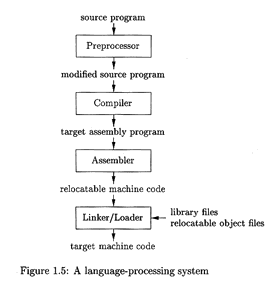
\includegraphics[scale = .95]{Language_Processing_System.png}
\caption{A language-processing system (taken from \cite{Aho:1986:CPT:6448})}
\label{fig:A language-processing system}
\end{figure}

specifically speaking, parts of a compiler (see Figure~\ref{fig:Phases of Compiler}).

\begin{figure}[th]
\centering
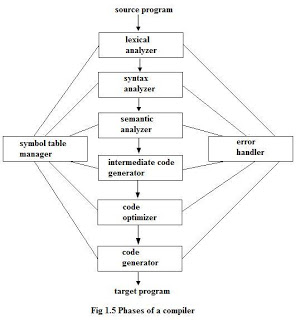
\includegraphics[scale = 0.7]{Phases_of_compiler.jpg}
\caption{Phases of Compiler \cite{Aho:1986:CPT:6448}}
\label{fig:Phases of Compiler}
\end{figure}

The architecture for a compiler as described in Figure~\ref{fig:Phases of Compiler} is not needed
since \progLang{Haskell} provides most of
them.
Nonetheless, the library has the following major components,\eref{comma-before-list}

\begin{enumerate}
\item Syntax, defining the language.

\item Database, to create a storage for the expressions.

\item Parser.

\item Interpreter.

\item Unifier.

\item Read-Eval-Print Loop\Verb[showspaces]! !(REPL).\endnote{%
  Fix the preceding space.
}
\end{enumerate}

To prove the modularity of the approach for language modification and monadic unification only the abstract syntax
and unifier will be customized.\endnote{%
  Page break following removed.
}



\section{What we do in this prototype?}

\begin{comment}
In the first prototype we just did unification of two terms not query resolution.

We do complete \progLang{Prolog} query resolution like stuff.

\ref{proto1} provides a generic procedure / methodology to convert a language into monadic unifiable form
\end{comment}


Unification is a part of the \progLang{Prolog} working. Simply speaking unification tells us whether or not two terms can be made equal.
The other part is to reach to a point in time when two terms are gathered depending upon matching rules in the knowledge base. This is where
a search strategy comes into play along with a backtracking mechanism.

Putting everything together forms the \progLang{Prolog} query resolver. Given a query and a knowledge, the query resolver matches the
input query with the rules in the knowledge base to create a list of goals to satisfy to generate an unifier along with saving choice
points on the way for backtracking.

This chapter discusses about how the abstract syntax and query resolver from \cite{prolog-lib} can be adapted to the concepts and
implementation from Chapter~\ref{proto1}. This not only proves how generic and modular the approach from the previous chapter is but also
the system working as a whole.\endnote{%
  Page break following removed.
}



\section{Current implementation (prolog-0.2.0.1)}

Beginning with language from Figure~\ref{tab:origgramp0201} is transformed into an isomorphically equivalent
grammar described in Figure~\ref{tab:flatgrp0201}.

\begin{code-list}[h]
  \begin{singlespace}
    \inputminted[linenos]{haskell}{haskell-proto2-flattened-rarefy.hs}
  \end{singlespace}
  \caption{Flattened (non-recursive) grammar}
\label{tab:flatgrp0201}
\end{code-list}


After the language is opened up, the next step is to replace the current unification procedure to the one {\Huge
  ?\endnote{%
  Something is missing here.  The current text comes from commit \texttt{a1b2c01fb24}.
}}


The current unification uses basic pattern matching to unify the terms. All the shortcomings related to the language also affect the
unification mechanism.

Beginning with the result produces by the query resolver shown in Figure~\ref{tab:prlg0201unifier}.
\begin{code-list}[h]
\begin{minted}[linenos]{haskell}
type Unifier      = [Substitution]
type Substitution = (VariableName, Term)
\end{minted}
\caption{prolog-0.2.0.1 Unifier}
\label{tab:prlg0201unifier}
\end{code-list}
A \markWord{Unifier} is a list of \markWord{Substitutions} which binds a variable to a value.

\begin{comment}
Figure~\ref{tab:prlg0201unifier} shows the result type. The instances are created to open up the language and make it compatible with the
unification library \cite{prolog-lib}.
\end{comment}

Coming back to the unification itself shown in Figure~\ref{tab:prlg0201unification}.
Each language expression is matched based on its structure.

\begin{code-list}[h]
  \begin{singlespace}
    \inputminted[linenos]{haskell}{haskell-proto2-unification-lion.hs}
  \end{singlespace}
\caption{prolog-0.2.0.1 Unification}
\label{tab:prlg0201unification}
\end{code-list}

The issue with the current approach is the rigidity of the procedure.
Any language modification will cause a ripple effect across the system.
As described in Chapter~\ref{proto1}, the advantages of \textit{functorizing} language hold in this implementation
as well.\endnote{%
  Page break following removed.
}

\begin{comment}
\section{Modifications}
The resulting language is not far from what we did in {\Large ?\LARGE ?}~\ref{proto1}\endnote{%
  Fix me!
}
apart from the fact that the \markWord{Term} expressions are encapsulated
to form \markWord{Clauses} which in turn form a \markWord{Program}.

Moreover, the required instances make the language compatible with the unification procedure.

\begin{singlespace}
  \inputminted[linenos]{haskell}{haskell-proto2-starry-forked.hs}
\end{singlespace}

Aditionally helper functions for converting expressions between the two domains and translation to \markWord{UTerm}.

To solve the issue of infinitely deep language expressions, we find the fixed point of the expression.
The unification function provided by \cite{prolog-lib} is not very \progLang{Prolog} like\eref{language-like} in
nature and certain adjustments need to be made.
\begin{enumerate}
\item Extracting variable and creating dictionaries.

\item Converting to \markWord{UTerm}s and back
\end{enumerate}

\begin{singlespace}
  \inputminted[linenos]{haskell}{haskell-proto2-clean-lemur.hs}
\end{singlespace}

Take original expressions flatten fix convert unify
run it \markWord{STBinding} monad to extract substitutions.\endnote{%
  Huh?
}

\begin{singlespace}
  \inputminted[linenos]{haskell}{haskell-proto2-hearty-kayo.hs}
\end{singlespace}
\end{comment}



\section{Results}

It works\yyy{,}{.}



\section{Chapter Recapitulation}

\ifMain
\begin{scope}
  \nolinenumbers
  \enotesize
  \par
  \begin{singlespace}
  \setlength{\parskip}{12pt plus 2pt minus 1pt}
  \theendnotes
  \par
  \end{singlespace}
\end{scope}
\unbcbibliography{bibliography}
\fi

\end{document}
